\documentclass[12pt, svn, draft]{rureport}
\svnid{$Id: example-techreport.tex 48 2014-10-23 15:40:52Z foley $}
\svnidlong{$HeadURL: https://projects.cs.ru.is/projects/t-411-mech-2014/repository/changes/group/DataCollector/FinalReport/GeoLog.tex $}
{$LastChangedDate: 2014-10-23 15:40:52 +0000 (Thu, 23 Oct 2014) $}
{$LastChangedRevision: 48 $}
{$LastChangedBy: foley $}
% if you'd like the above information to be updated,
% use svn properties to set svn:keywords to for Id and URL (or HeadURL)
% Don't forget to set the draft to final before submitting

\author{Páll Helgason pallsh12@ru.is\\Sindri Ólafsson sindrio12@ru.is\\Sveinn Elmar Magnússon sveinnm12@ru.is\\Þór Tómasarson thortom12@ru.is}  % My name, for the titlepage
\title{Geo Log,\\ \large{data logger for geological research}}  % The title, for the titlepage
\shorttitle{Geo Log}
\course{T-411-MECH Mechatronics 1}
\instructor{Joe Foley}
% Change the graphics path if you are storing your graphics somewhere different
\graphicspath{{graphics/}{Graphics/}{./}}

\usepackage{subfiles}
\usepackage{float}
\usepackage{gensymb}

\begin{document} % this tells the compiler that it is time to make
                 % text to print instead of just getting ready.
\maketitle  % make a title page from the Title, Date, and Author
\tableofcontents
\pagebreak

\subfile{intro}
\pagebreak
\subfile{background}
\subfile{requirements}
\subfile{design}
\subfile{testing}
\subfile{usage}
\subfile{results}
\subfile{conclusion}

\pagebreak
\addcontentsline{toc}{section}{References}
\bibliographystyle{IEEEtran}
\bibliography{references}

\pagebreak
\addcontentsline{toc}{section}{Appendix}
\section*{Appendix}
\addcontentsline{toc}{subsection}{Design Documents}
\subsection*{Design documents}
%Put CAD drawings, additional sketches.  If there are many, it is better to put the high-level drawings (assemblies), then put the rest of the drawings somewhere that the reader can retreive them (SVN, etc.).  Don't forget to put a link here.

\begin{figure}[H]
\centering
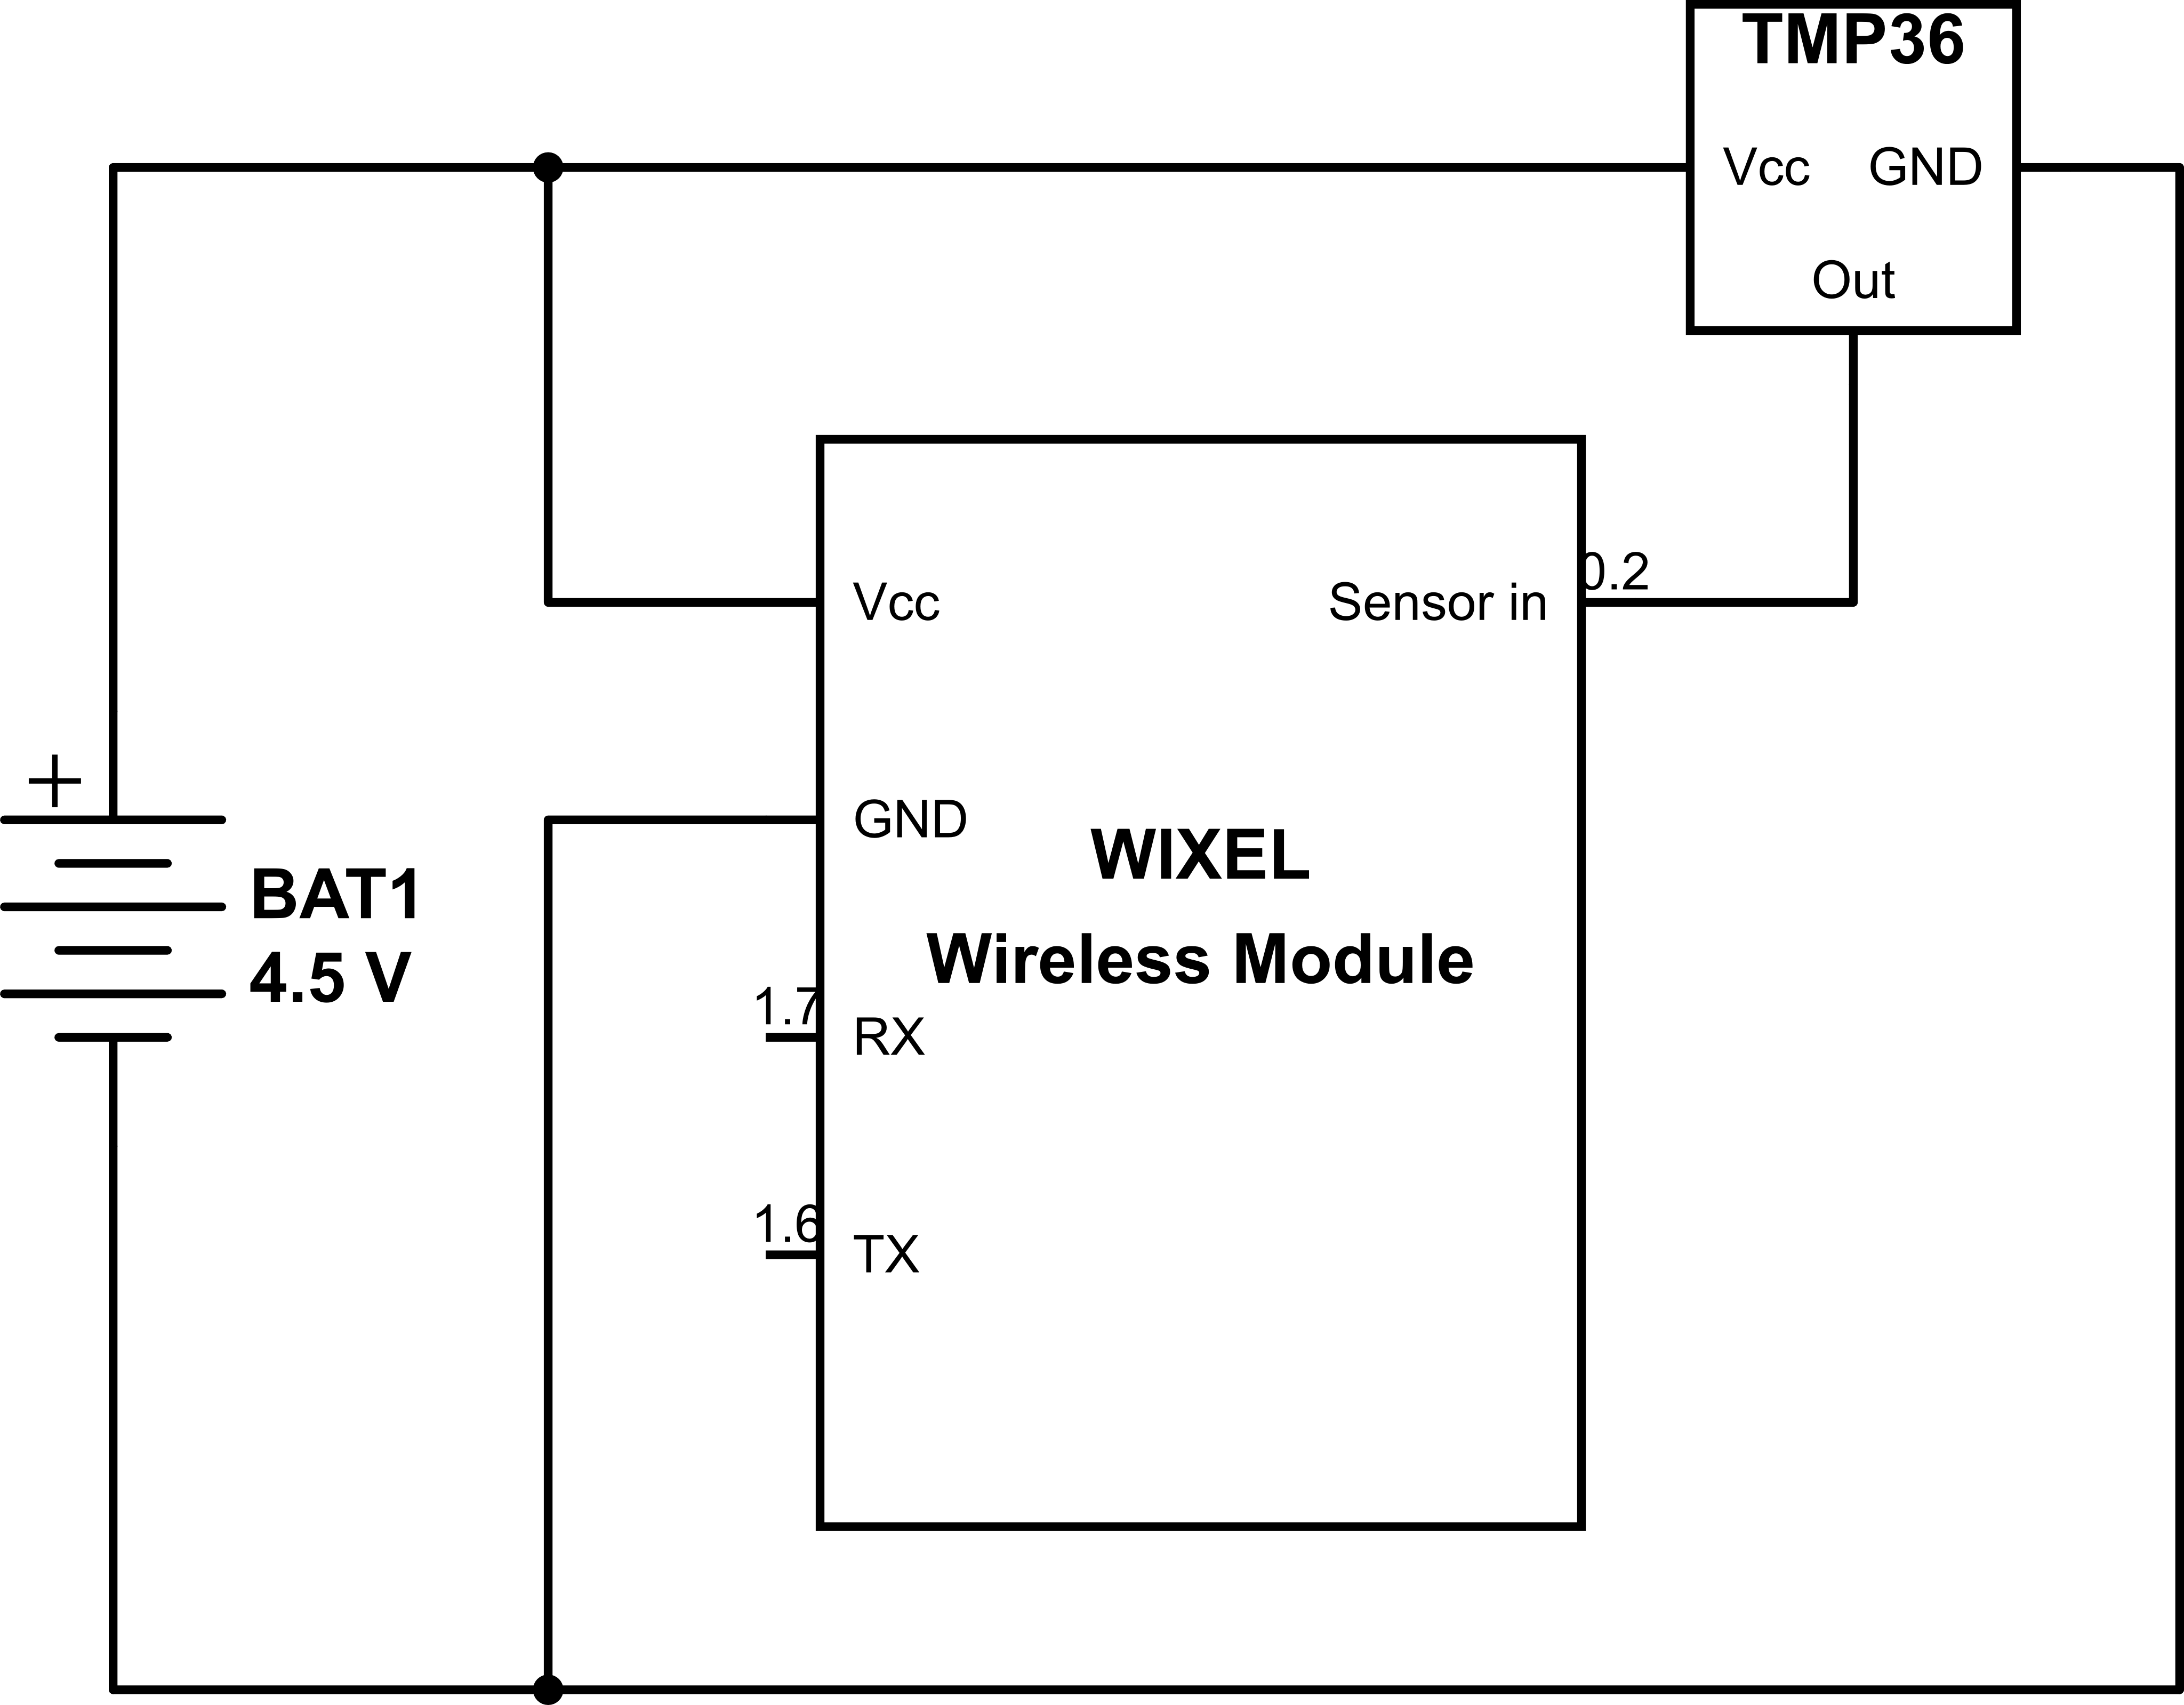
\includegraphics[width=0.5\linewidth]{graphics/sensormodule_schematic}
\caption{Electrical Schematic Diagram of the Wireless Sensor Module\label{fig:sensormodule_schematic}}
\end{figure}

\begin{figure}[H]
\centering
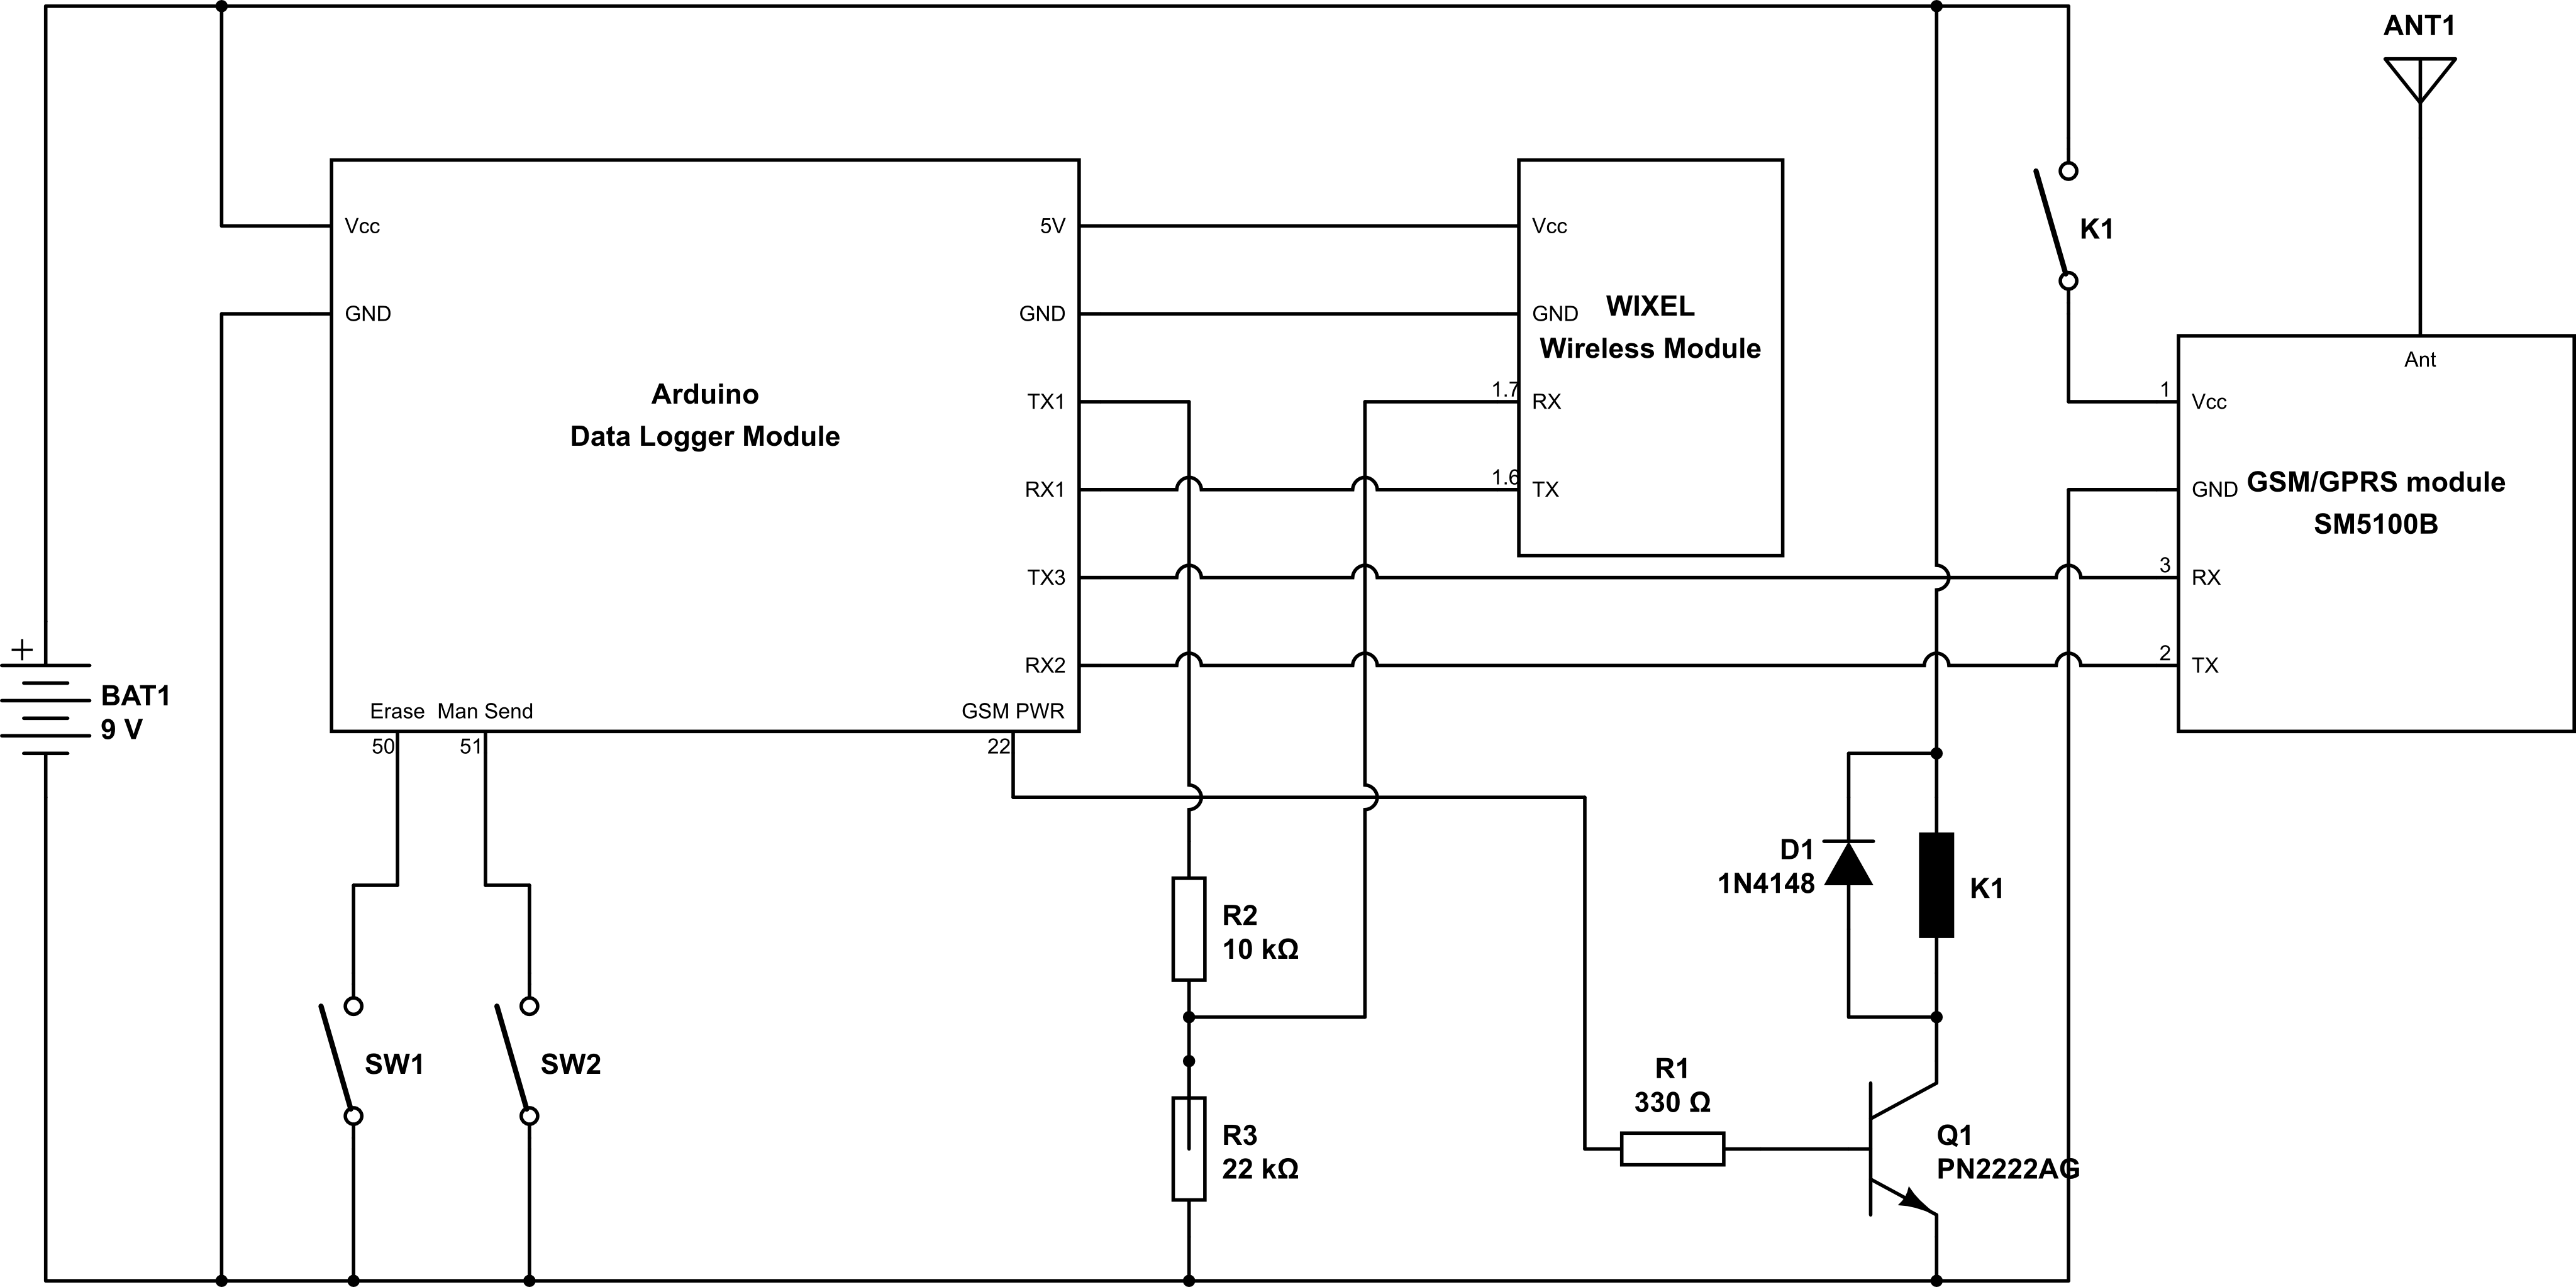
\includegraphics[width=1\linewidth]{graphics/motherhub_schematic}
\caption{Electrical Schematic Diagram of the Mother Hub\label{fig:motherhub_schematic}}
\end{figure}

\begin{figure}[H]
\centering
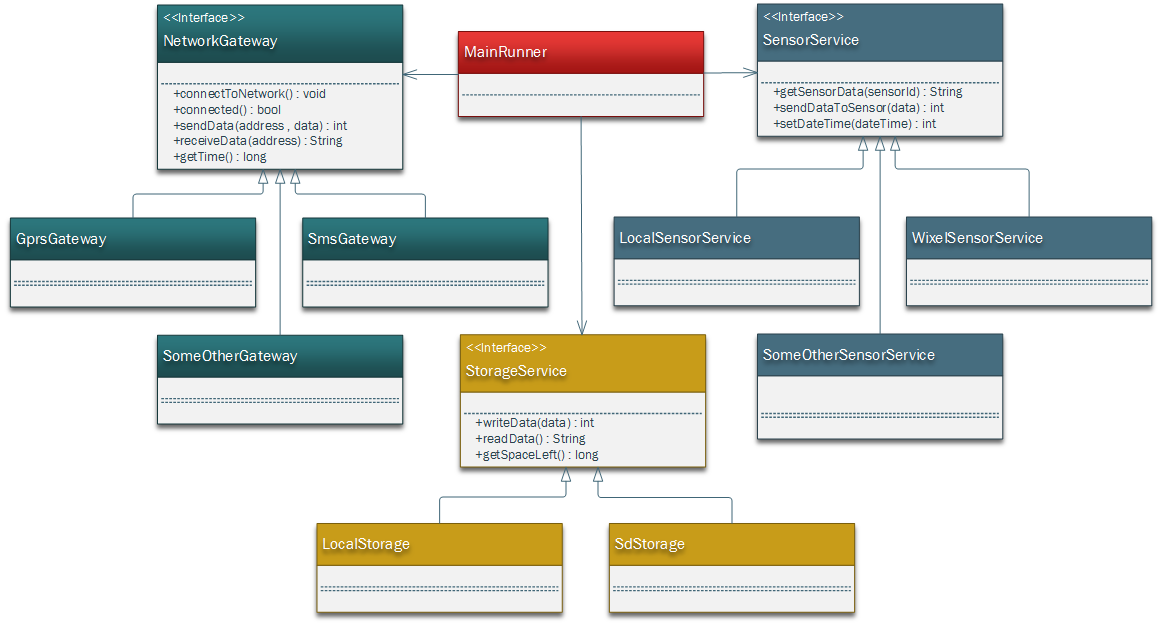
\includegraphics[width=1\linewidth]{graphics/ClassDiagram}
\caption{Class Diagram of the system\label{fig:ClassDiagram}}
\end{figure}



\end{document} % Ignore everything after this line (end the document)
